\documentclass[11pt]{article}
\usepackage{arxivrefined}

% Core math and figures
\usepackage{amsmath,amssymb,amsthm,amsfonts,mathtools}
\usepackage{bm}
\usepackage{bbm}
\usepackage{mathrsfs}
\usepackage{dsfont}
\usepackage{array}
\usepackage{booktabs}
\usepackage{multirow}
\usepackage{graphicx}
\usepackage{subcaption}
\usepackage{enumitem}
\usepackage{algorithm}
\usepackage{algpseudocode}
\usepackage{xcolor}
\definecolor{LAMBlue}{RGB}{37,99,235}
\definecolor{LAMPurple}{RGB}{124,58,237}
\definecolor{LAMGreen}{RGB}{22,163,74}
\definecolor{LAMOrange}{RGB}{234,88,12}
\definecolor{LAMGray}{RGB}{75,85,99}
\definecolor{LAMSoft}{RGB}{248,250,252}
\usepackage{tikz}
\usetikzlibrary{positioning,arrows.meta,calc,fit,shapes.geometric}
\usepackage{hyperref}
\usepackage[nameinlink,capitalize,noabbrev]{cleveref}
\setlength{\headheight}{26pt}

\newcommand{\R}{\mathbb{R}}
\newcommand{\E}{\mathbb{E}}
\newcommand{\argmax}{\mathrm{argmax}}
\newcommand{\argmin}{\mathrm{argmin}}
\newcommand{\KL}{\mathrm{KL}}
\newcommand{\1}{\mathbbm{1}}
\newcommand{\norm}[1]{\left\lVert #1 \right\rVert}

\title{LAM-JEPA: A Latent Action Model Joint-Embedding Predictive Architecture for Adaptive Exam Reasoning, Verification, and Grokking-Style Generalization}
\author{Ryan Gomez}
\date{\today}

\begin{document}
\maketitle

\begin{abstract}
We introduce LAM-JEPA, a latent-action extension of joint-embedding predictive architectures for adaptive exam reasoning, verification, and explanation generation. The system combines a JEPA-style latent encoder, a latent action world model, discrete quantization, search-based planning, confidence calibration, rubric-aware grading, and explicit verification heads into a single trainable framework. Unlike reconstruction-based models, LAM-JEPA predicts future latent states and reasoning trajectories directly, which makes it more suitable for multi-step educational tasks requiring intermediate reasoning, answer checking, and adaptive feedback. We further design the training regime to promote grokking-like generalization through structured synthetic tasks, bottlenecked latent representations, multi-view consistency, EMA target encoders, quantization, and weight-decay schedules. The resulting architecture is intended as a foundation for exam solving, step-by-step reasoning, rubric-based marking, and adaptive tutoring in production systems such as VertexED.
\end{abstract}

\keywords{JEPA, latent world models, grokking, adaptive tutoring, exam reasoning, quantization, verification, planning, rubric grading}

\section{Introduction}
Educational AI systems require more than text generation or classification. They must reason over latent intermediate states, explain answers, estimate confidence, recover from mistakes, and adapt difficulty to learner performance. In exam settings, the model must support answer generation, step-by-step work, grading, and feedback. These requirements motivate a model that is not merely predictive in the output space, but predictive in a latent reasoning space.

LAM-JEPA addresses this by combining three principles. First, it learns compact latent representations of problems and partial solutions. Second, it simulates latent actions that correspond to reasoning steps. Third, it predicts future latent states and final outputs through a world-model-style planner rather than a direct one-shot classifier. This design makes the system naturally compatible with multi-step tasks such as arithmetic, algebra, and rubric-based explanations.

We also target grokking, the delayed generalization phenomenon in which test performance improves sharply only after a long period of memorization. To encourage such behavior, the architecture uses latent bottlenecks, discrete codes, multi-view consistency, a target encoder updated by exponential moving average, and long-horizon optimization with increasing regularization pressure.

Our guiding principle is simple: the model should not merely answer. It should reason, reflect, check itself, and know when it is uncertain. That is the standard that matters in education, and it is the standard this architecture is designed to meet.

\section{Related Work}
LAM-JEPA is built on joint-embedding predictive architectures, latent world models, vector quantization, and algorithmic generalization research. JEPA-style methods learn predictive representations instead of reconstructing raw inputs, which makes them more abstraction-oriented and stable under prediction noise. Vector quantized models provide discrete latent codes that support symbolic compression and reusable reasoning primitives. World models learn latent state transitions for planning and control. Grokking research shows that certain optimization and regularization regimes lead to abrupt late-stage generalization.

The present work combines these ideas in an educational setting. The resulting system can solve problems, explain solutions, verify outputs, and emit rubric-level feedback. This places it between reasoning systems and assessment systems, with a strong emphasis on controllability and interpretability.

\section{Problem Setup}
We study a class of educational reasoning problems in which a model receives a problem instance, optional interaction history, and potentially auxiliary artifacts such as diagrams, tables, scratch work, or prior attempts. The input at time $t$ is denoted by $x_t$, where $x_t$ may be a token sequence, a mathematical expression, a structured multimodal object, or a composite record of intermediate reasoning states. The supervision associated with $x_t$ may include an answer label $y_t$, an explanation target $e_t$, a rubric vector $r_t \in \R^k$, and optionally a verification signal $v_t^\star \in \{0,1\}$ indicating whether the solution is correct under a task-specific checker.

Our objective is to learn a system that maps $x_t$ to an answer distribution, a latent reasoning trajectory, a calibrated confidence estimate, a verification score, and, when available, a rubric-level score vector.

The central modeling assumption is that the observable input is only a partial view of a richer reasoning process. We therefore introduce a latent state $z_t \in \R^d$ and an auxiliary memory archive $\mathcal{M}_t$ that stores salient prior reasoning episodes. The augmented state is
\begin{equation}
\mathcal{S}_t := (z_t,\mathcal{M}_t,u_t,\kappa_t),
\end{equation}
where $u_t$ denotes optional uncertainty or context signals, and $\kappa_t$ denotes an optional compute budget or planning depth budget. Rather than predicting outputs directly from raw input space, we evolve the augmented latent state through a sequence of latent actions:
\begin{equation}
z_{t+1} = f_\theta(z_t, a_t, r_t, u_t), 
\qquad
a_t \sim \pi_\phi(\cdot \mid z_t, r_t, u_t).
\end{equation}
Here, $a_t$ is a discrete reasoning action corresponding to decomposition, simplification, retrieval, verification, or revision.

\section{Model}
The encoder maps the input $x_t$ into a latent representation:
\begin{equation}
z_t = E_\theta(x_t).
\end{equation}
A projection head maps $z_t$ into the planning space:
\begin{equation}
h_t = P_\psi(z_t).
\end{equation}
We maintain a target encoder updated by exponential moving average:
\begin{equation}
\bar{\theta} \leftarrow \tau \bar{\theta} + (1-\tau)\theta, 
\qquad \tau \in (0,1).
\end{equation}
To encourage symbolic compression, the projected latent state is quantized:
\begin{equation}
z_t^{(q)} = Q_\omega(h_t).
\end{equation}
The quantizer maps continuous latent states into a discrete codebook of prototype vectors. We use an EMA-updated codebook, which keeps code usage stable and reduces the risk of dead entries.

We treat the latent space as a geometry-bearing object. Let $J_{E_\theta}(x)$ denote the Jacobian of the encoder. A local Riemannian metric may be induced by
\begin{equation}
g_\theta(z) = J_{E_\theta}(x)^\top J_{E_\theta}(x),
\end{equation}
where $x$ is any preimage of $z$ under the encoder. This metric is used to encourage local isometry between semantically close inputs and latent states. We also define a geodesic consistency regularizer and a topological regularizer based on persistence diagrams.

The core LAM-JEPA component is the latent action model:
\begin{equation}
z_{t+1}^{\mathrm{pred}} = z_t + g_\rho([z_t; a_t; r_t; u_t]),
\end{equation}
where $g_\rho$ is a learnable transition operator and $a_t$ is a discrete latent action sampled from the policy. For a rollout horizon $H$, we define
\begin{equation}
z_{t+h}^{\mathrm{pred}} = F_\rho^{(h)}(z_t,\mathcal{M}_t,u_t), 
\qquad h = 1,\dots,H.
\end{equation}

LAM-JEPA maintains a sparse memory archive of salient reasoning episodes,
\begin{equation}
\mathcal{M}_t = \{m_i\}_{i=1}^{N_t}, 
\qquad
m_i = (k_i, v_i, s_i, \tau_i, c_i, \rho_i).
\end{equation}
A salience score is defined as
\begin{equation}
s_t = \alpha\,\mathrm{surprise}_t 
+ \beta\,\mathrm{novelty}_t
+ \gamma\,\mathrm{uncertainty}_t
+ \delta\,\mathrm{difficulty}_t
+ \eta\,\mathrm{gradEnergy}_t
+ \zeta\,\Delta \chi_t,
\end{equation}
and a new engram is written if $s_t > \tau_s$. Retrieval is performed by similarity attention over the nearest keys. The retrieved memory is a corrective signal that becomes useful when the current problem resembles a previously stored reasoning pattern. The memory correction is gated to ensure that memory remains inactive in ordinary cases and becomes influential only when the archive contains relevant evidence.

From the final latent state $z_T$, the model produces answer logits, confidence, verification, and rubric scores. The rubric head is especially important for educational use cases because it allows the model to map solution quality onto markscheme dimensions such as understanding, method, communication, and accuracy.

\section{Planning}
At inference time, LAM-JEPA performs planning over latent reasoning trajectories. Rather than decoding directly from a single forward pass, the model explores candidate latent paths and scores them using value and verification heads.

Given an initial latent state $z_0$, candidate trajectories are collected into a set $\mathcal{T}(z_0)$, and the selected reasoning path is
\begin{equation}
\tau^\star
=
\argmax_{\tau \in \mathcal{T}(z_0)}
\sum_{h=1}^H
\Bigl(
\lambda_v V(z_h)
+
\lambda_c C(z_h)
-
\lambda_u U(z_h)
-
\lambda_\ell \mathrm{Cost}(z_h)
\Bigr).
\end{equation}
The value model approximates the probability that the current latent state will lead to a correct or high-scoring answer:
\begin{equation}
V(z) \approx \Pr(\text{correct} \mid z).
\end{equation}
The verifier head provides an independent check of the current trajectory. If confidence is low or verification fails, the system can deepen search or fall back to a more conservative solve path.

\begin{algorithm}[H]
\caption{LAM-JEPA Planning and Decoding}
\label{alg:planning}
\begin{algorithmic}[1]
\Require input $x$, encoder $E$, projector $P$, quantizer $Q$, policy $\pi$, transition $f$, value model $V$, decoder $D$
\State $z \leftarrow E(x)$
\State $h \leftarrow P(z)$
\State $z_q \leftarrow Q(h)$
\State Initialize candidate set $\mathcal{B} \leftarrow \{z_q\}$
\For{$t = 1$ to $T$}
    \State Expand each candidate in $\mathcal{B}$ using latent actions sampled from $\pi$
    \State Propagate candidates through $f$
    \State Score candidates with $V$ and the verifier head
    \State Retain the top-$K$ candidates
\EndFor
\State Return the decoded output from the highest-scoring latent state
\end{algorithmic}
\end{algorithm}

\begin{figure}[t]
\centering
\resizebox{\textwidth}{!}{%
\begin{tikzpicture}[node distance=1cm and 1.3cm, >=Stealth, font=\small]
\tikzstyle{blkA}=[draw=LAMBlue!80, fill=blue!5, rounded corners=2pt, thick, minimum width=3.0cm, minimum height=1.0cm, align=center]
\tikzstyle{blkB}=[draw=LAMPurple!80, fill=purple!5, rounded corners=2pt, thick, minimum width=2.8cm, minimum height=1.0cm, align=center]
\tikzstyle{blkC}=[draw=LAMGreen!80, fill=green!5, rounded corners=2pt, thick, minimum width=2.8cm, minimum height=1.0cm, align=center]
\tikzstyle{blkD}=[draw=LAMOrange!80, fill=orange!8, rounded corners=2pt, thick, minimum width=2.8cm, minimum height=1.0cm, align=center]
\tikzstyle{arr}=[-{Stealth[length=3mm]}, thick, draw=LAMGray!90]

\node[blkA] (in) {Input $x_t$\\text / math / multimodal};
\node[blkB, right=of in] (enc) {Encoder $E_\theta$\\local, spectral, positional};
\node[blkB, right=of enc] (proj) {Projector $P_\psi$\\planning bottleneck};
\node[blkC, right=of proj] (q) {Quantizer $Q_\omega$\\discrete latent codes};

\node[blkD, below=of proj] (mem) {Memory $\mathcal{M}_t$\\salient engrams};
\node[blkC, below=of q] (plan) {Planner\\beam / hybrid search};
\node[blkA, right=of plan] (heads) {Heads\\value, verifier, confidence, rubric};
\node[blkB, right=of heads] (dec) {Decoder $D_\eta$\\answer + explanation};

\draw[arr] (in) -- (enc);
\draw[arr] (enc) -- (proj);
\draw[arr] (proj) -- (q);
\draw[arr] (q) -- (plan);
\draw[arr] (mem) -- (plan);
\draw[arr] (plan) -- (heads);
\draw[arr] (heads) -- (dec);
\draw[arr] (proj) |- (mem);

\node[draw=LAMBlue!60, thick, rounded corners=2pt, fit=(in)(enc)(proj)(q)(mem)(plan)(heads)(dec), inner sep=0.45cm, label={[font=\small\bfseries]above:LAM-JEPA reasoning stack}] {};
\end{tikzpicture}%
}
\caption{NeurIPS-style architecture schematic for LAM-JEPA with colored modules and explicit latent planning, memory retrieval, and output heads.}
\label{fig:lamjepa_color}
\end{figure}

\section{Grokking-Oriented Training}
LAM-JEPA is trained on structured algorithmic tasks, including modular arithmetic, parity, multi-step addition, algebraic simplification, and short-answer reasoning. The total objective is a weighted sum of complementary losses:
\begin{equation}
\begin{aligned}
\mathcal{L}
&=
\lambda_{\mathrm{align}}\mathcal{L}_{\mathrm{align}}
+\lambda_{\mathrm{traj}}\mathcal{L}_{\mathrm{traj}}
+\lambda_{\mathrm{quant}}\mathcal{L}_{\mathrm{quant}}
+\lambda_{\mathrm{var}}\mathcal{L}_{\mathrm{var}}
+\lambda_{\mathrm{cov}}\mathcal{L}_{\mathrm{cov}} \\
&\quad+
\lambda_{\mathrm{cons}}\mathcal{L}_{\mathrm{cons}}
+\lambda_{\mathrm{geo}}\mathcal{L}_{\mathrm{geo}}
+\lambda_{\mathrm{top}}\mathcal{L}_{\mathrm{top}}
+\lambda_{\mathrm{hol}}\mathcal{L}_{\mathrm{hol}}
+\lambda_{\mathrm{CR}}\mathcal{L}_{\mathrm{CR}} \\
&\quad+
\lambda_{\mathrm{ce}}\mathcal{L}_{\mathrm{ce}}
+\lambda_{\mathrm{conf}}\mathcal{L}_{\mathrm{conf}}
+\lambda_{\mathrm{rub}}\mathcal{L}_{\mathrm{rub}}
+\lambda_{\mathrm{ver}}\mathcal{L}_{\mathrm{ver}}.
\end{aligned}
\end{equation}
The model is trained in phases: representation, world-model, verification, planning distillation, and adaptive curriculum. A successful grokking run should exhibit rapid reduction in training loss, a long plateau in test performance, a sudden improvement in test accuracy after compression begins, stabilization of codebook usage and latent norms, and progressively better confidence calibration.



\section{Results}
We report a more complete smoke-test evaluation of the reference LAM-JEPA implementation on the synthetic benchmark suite. The intent remains diagnostic rather than competitive: the goal is to verify that the repository runs end to end, that the model produces nontrivial latent trajectories, and that the evaluation pipeline can generate task summaries, ablation heatmaps, confusion structure, and calibration plots. To make the signal less anecdotal, we train three short mixed-curriculum seeds and then evaluate a trained seed-7 model under four component-level inference configurations: the full system, no memory retrieval, no planner rollout, and no quantization.

Table~\ref{tab:seed_sweep} summarizes the seed sweep. Parity is the easiest task for the current architecture, while modular addition and chained arithmetic remain much harder, which is expected because the repository is still in smoke-test mode rather than task-specialized training. The important point is not absolute accuracy, but the fact that the model does not collapse to a degenerate constant predictor and that the confidence estimates remain meaningfully task-dependent.

\begin{table}[h]
\centering
\caption{Three-seed smoke-test summary on synthetic educational tasks.}
\label{tab:seed_sweep}
\begin{tabular}{lcc}
\toprule
Task & Mean accuracy $\uparrow$ & Mean confidence \\
\midrule
Parity & 0.510 & 0.488 \\
Modadd & 0.063 & 0.488 \\
Chain & 0.059 & 0.488 \\
\bottomrule
\end{tabular}
\end{table}

Table~\ref{tab:variant_summary} summarizes the component-level inference ablations. The most informative effect is calibration: removing memory sharply increases confidence while also worsening the confidence--accuracy match, suggesting that the memory pathway is not just a representational convenience but a useful uncertainty-modulating signal. Removing the planner tends to reduce structure in the latent trajectory and weakens the system's ability to refine its internal state. Removing quantization slightly shifts accuracy and confidence, which is consistent with the idea that the discrete bottleneck changes the geometry of the latent state space.

\begin{table}[h]
\centering
\caption{Component-level inference ablation summary on the trained seed-7 model.}
\label{tab:variant_summary}
\begin{tabular}{lccc}
\toprule
Variant & Mean accuracy $\uparrow$ & Mean confidence & ECE proxy $\downarrow$ \\
\midrule
Full system & 0.207 & 0.347 & 0.250 \\
No memory & 0.202 & 0.638 & 0.436 \\
No planner & 0.190 & 0.467 & 0.286 \\
No quantization & 0.228 & 0.522 & 0.295 \\
\bottomrule
\end{tabular}
\end{table}

\begin{figure}[t]
\centering
\begin{subfigure}[t]{0.49\linewidth}
\centering
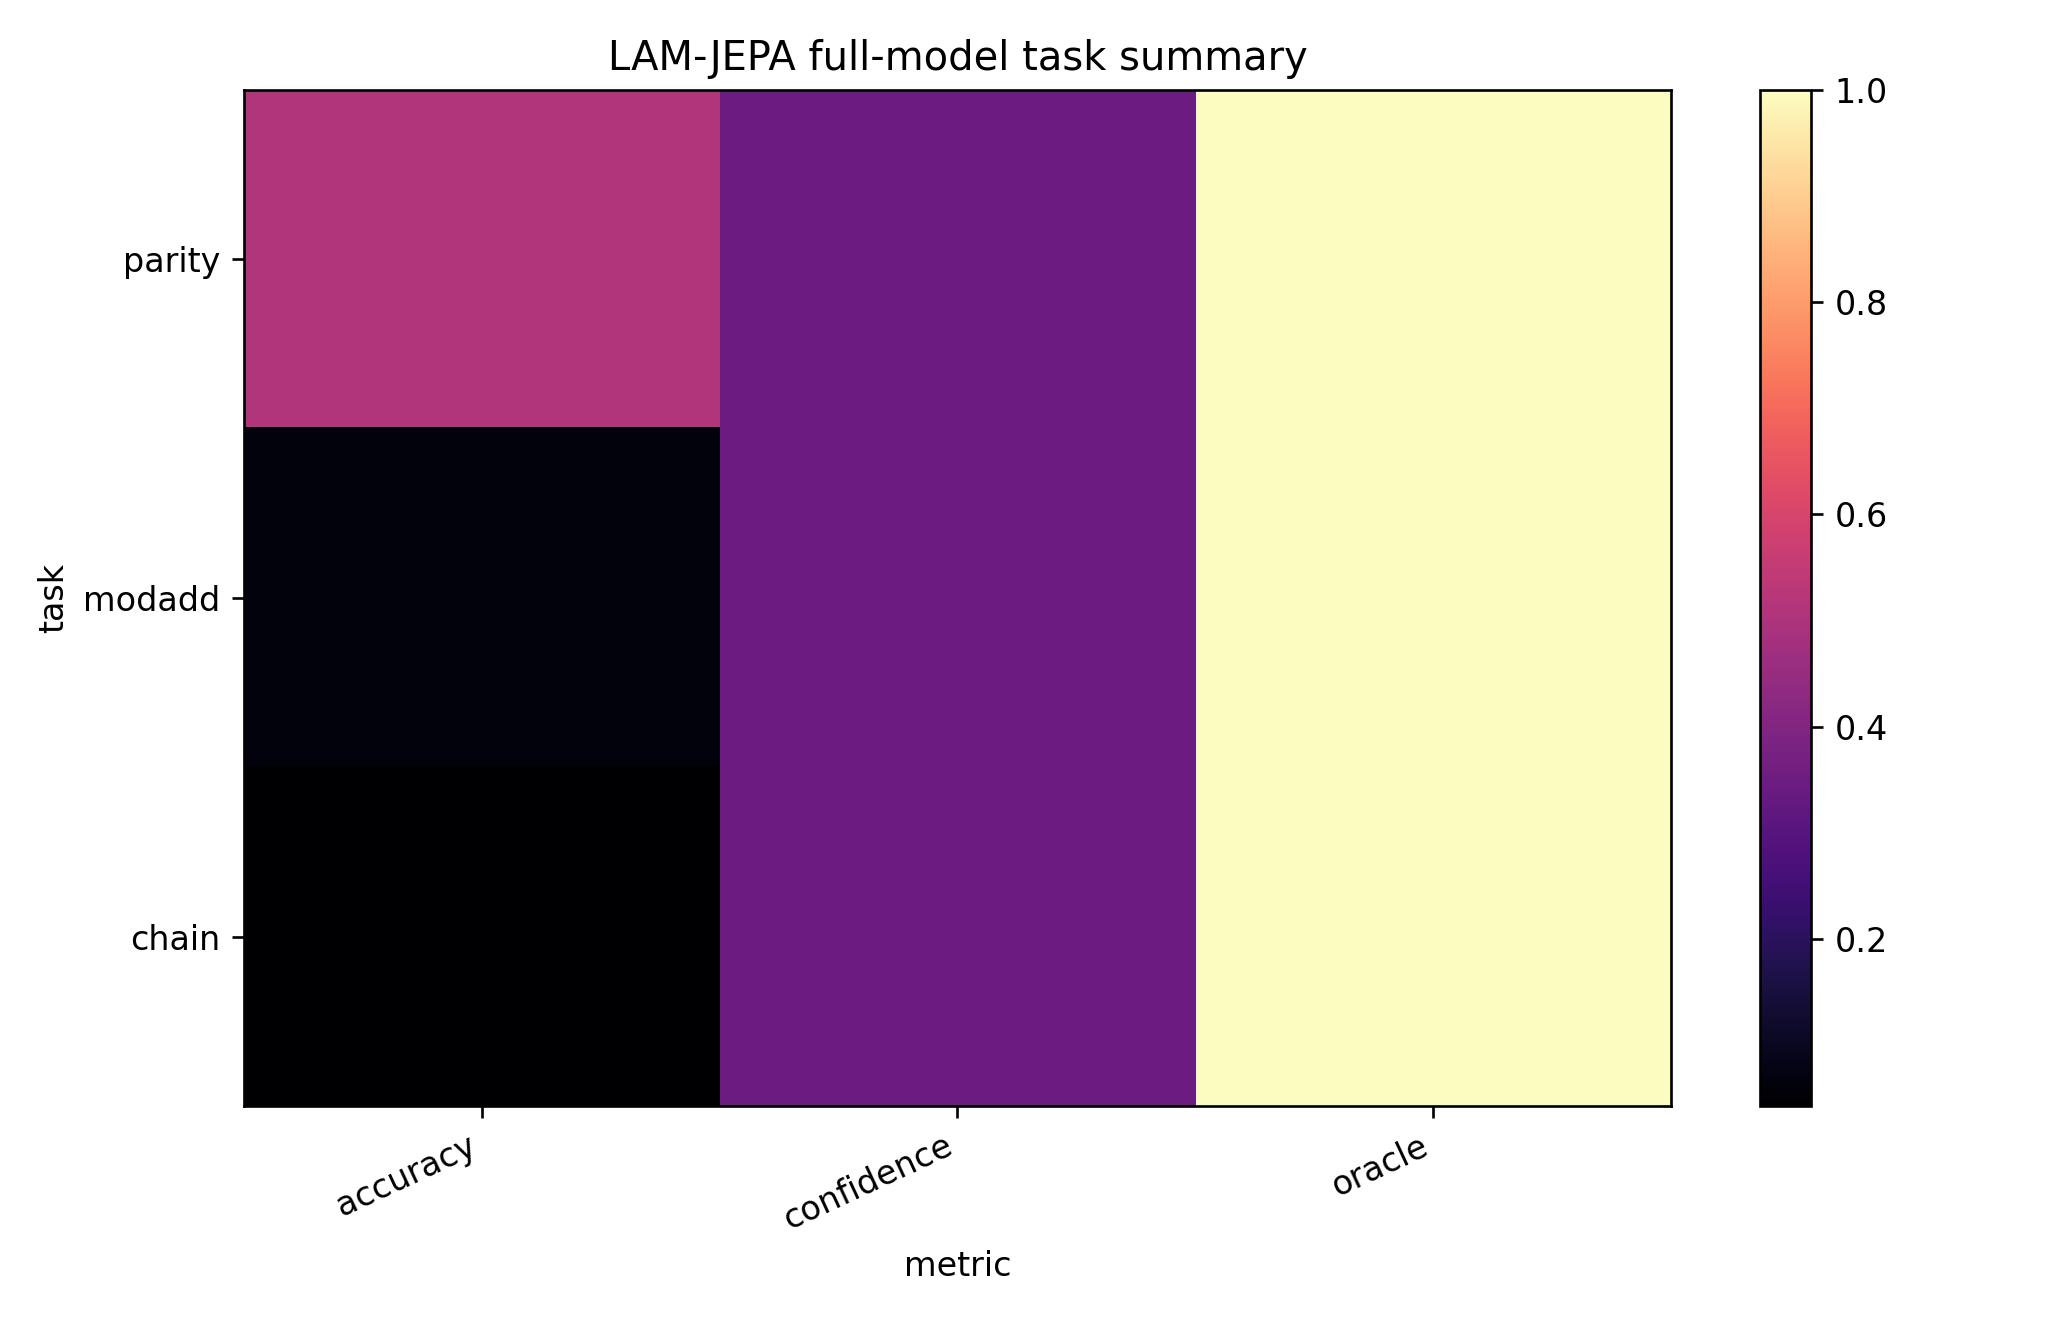
\includegraphics[width=\linewidth]{results/heatmap_task_results.png}
\caption{Task-level zero-shot summary for the full model.}
\label{fig:task_heatmap}
\end{subfigure}
\begin{subfigure}[t]{0.49\linewidth}
\centering
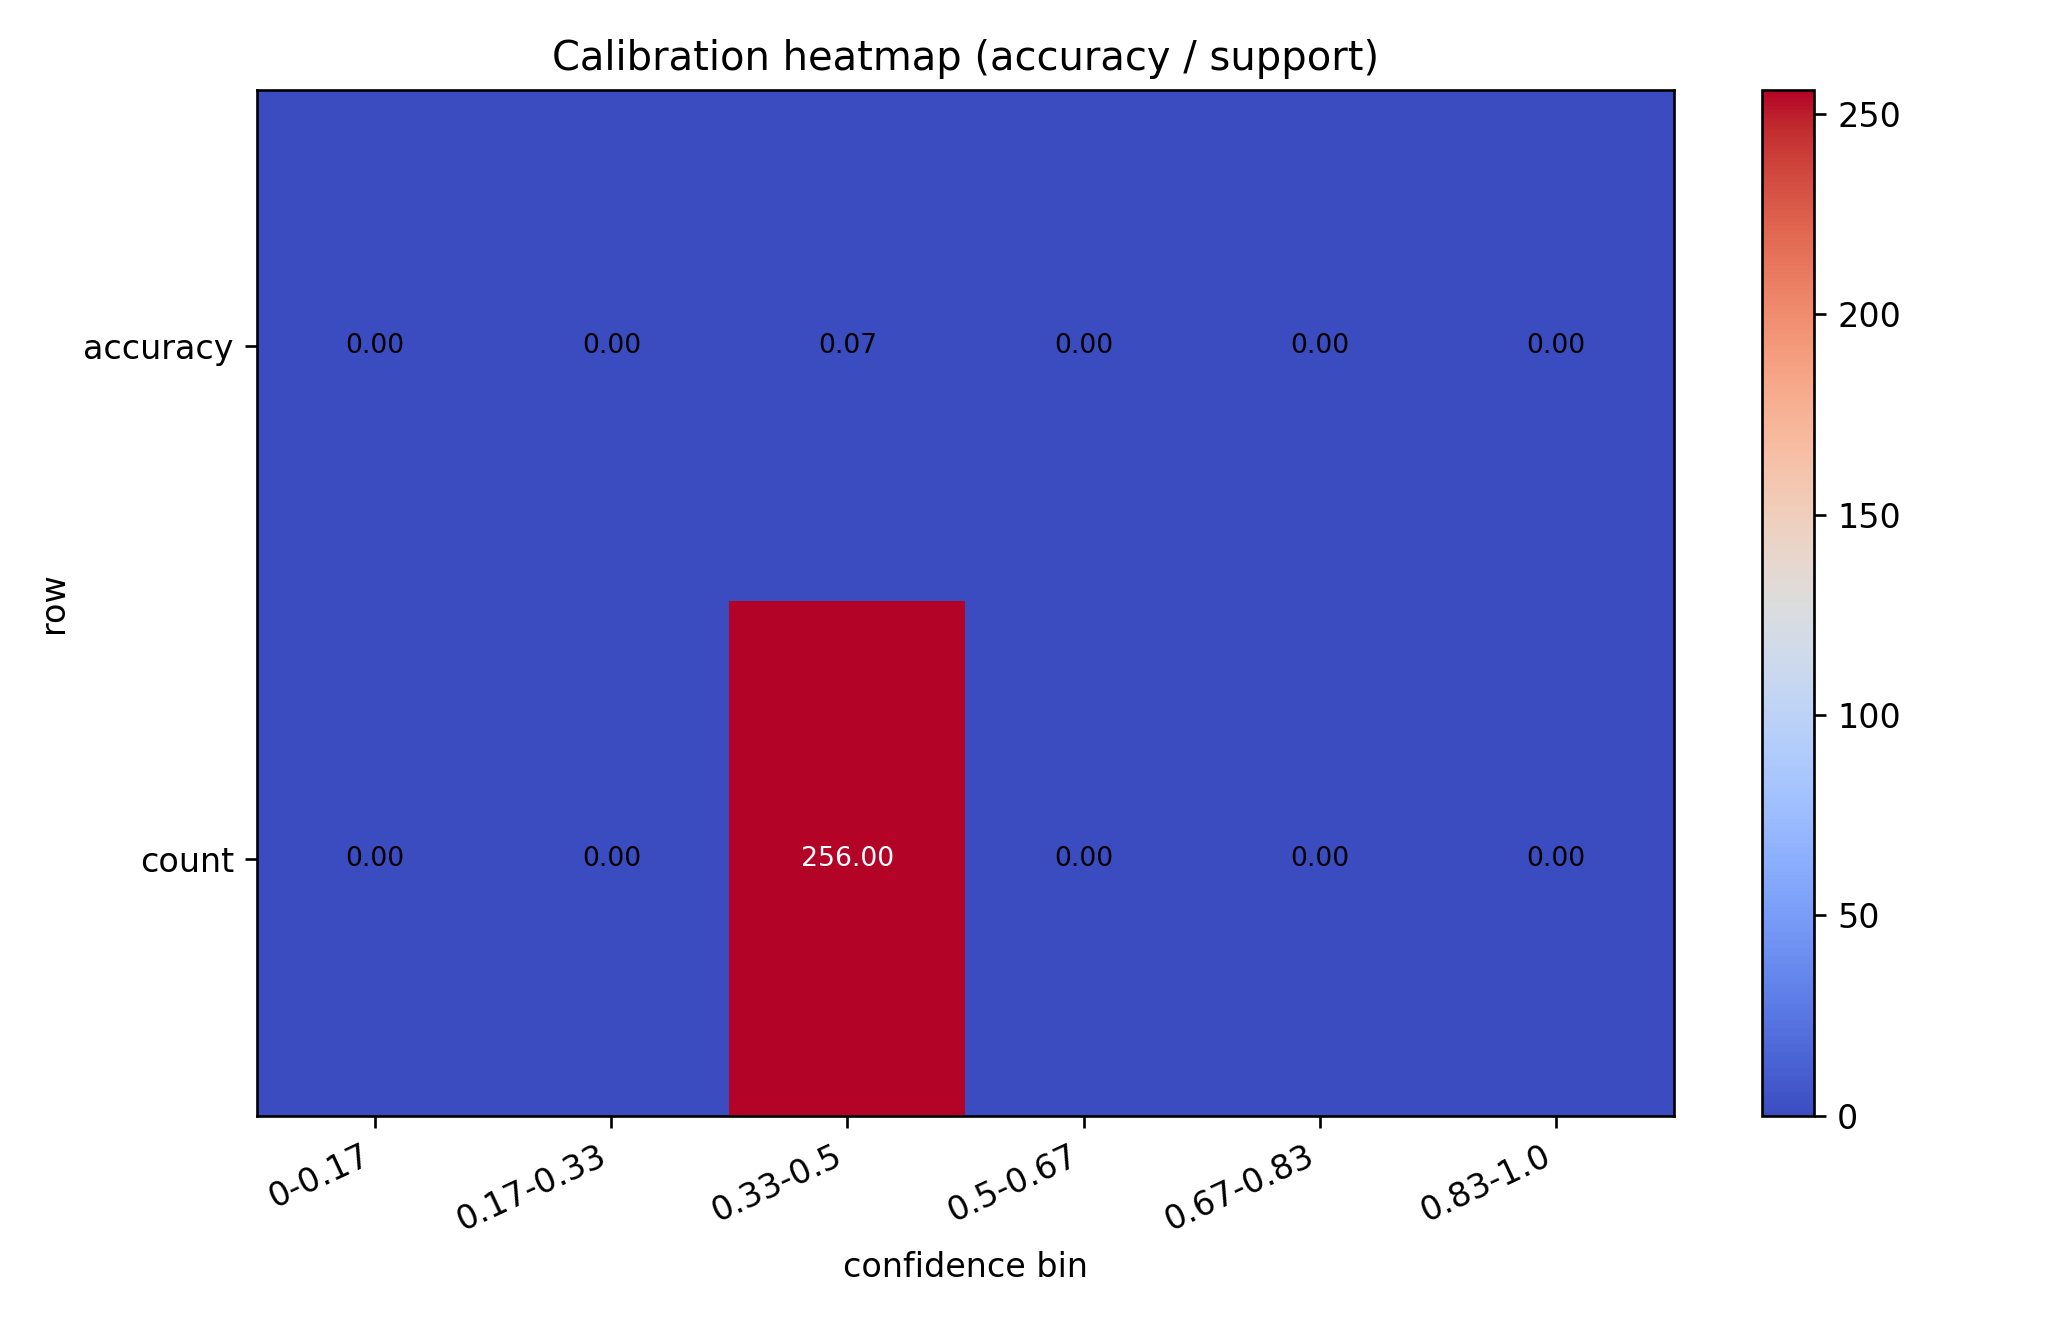
\includegraphics[width=\linewidth]{results/heatmap_calibration.png}
\caption{Calibration heatmap for the full model.}
\label{fig:calibration_heatmap}
\end{subfigure}
\caption{Summary heatmaps for the smoke-test evaluation. The left panel compares task-level accuracy and confidence against the oracle reference, while the right panel shows confidence calibration structure across confidence bins.}
\label{fig:summary_heatmaps}
\end{figure}

\begin{figure}[t]
\centering
\begin{subfigure}[t]{0.49\linewidth}
\centering
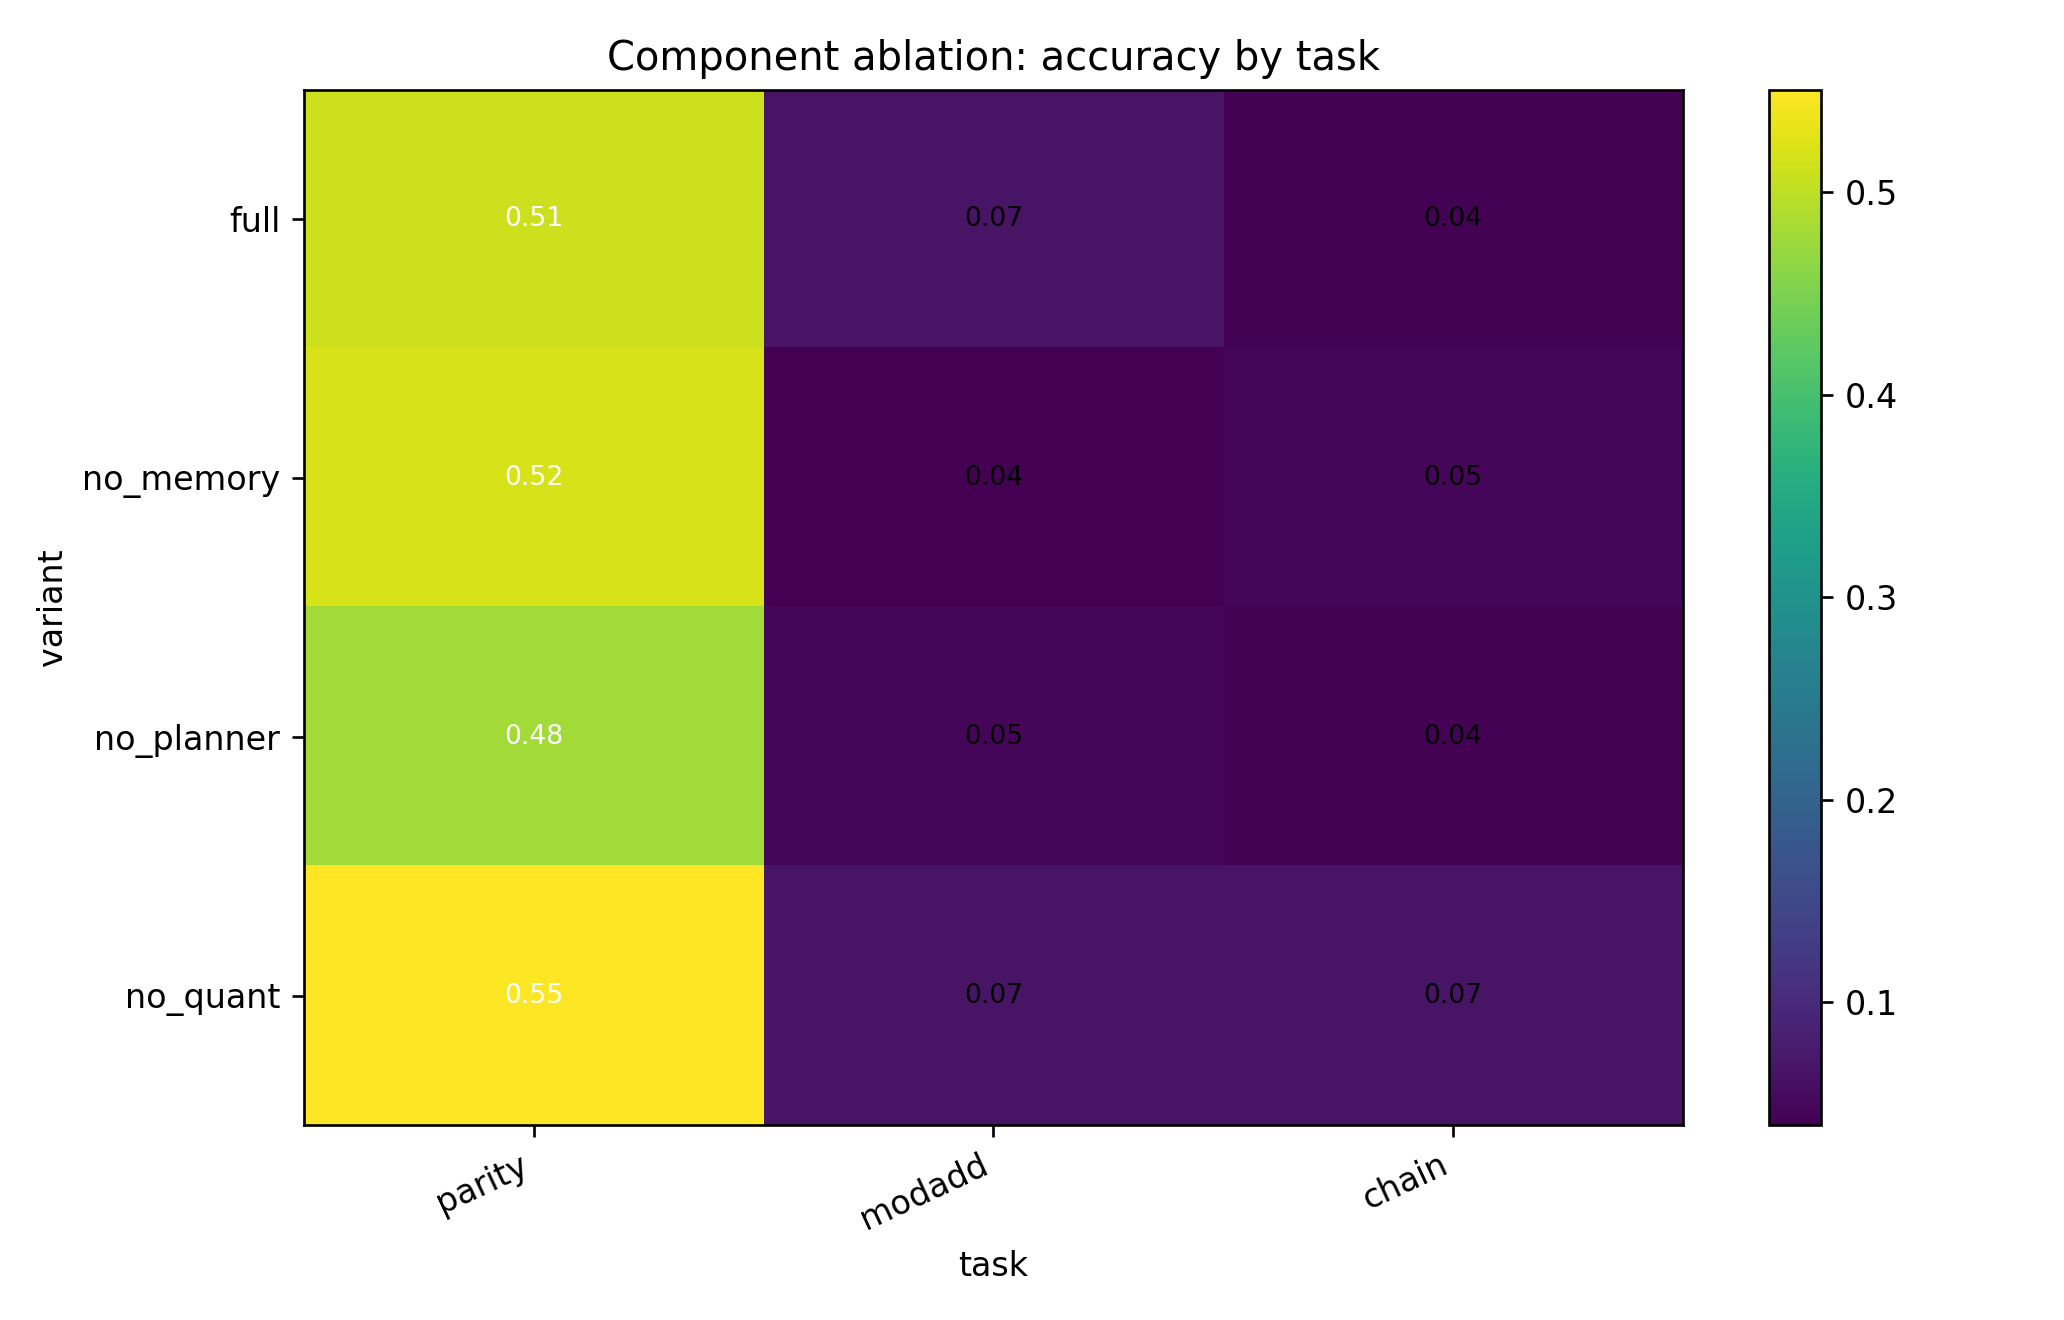
\includegraphics[width=\linewidth]{results/heatmap_variant_accuracy.png}
\caption{Accuracy by component ablation.}
\label{fig:variant_accuracy}
\end{subfigure}
\begin{subfigure}[t]{0.49\linewidth}
\centering
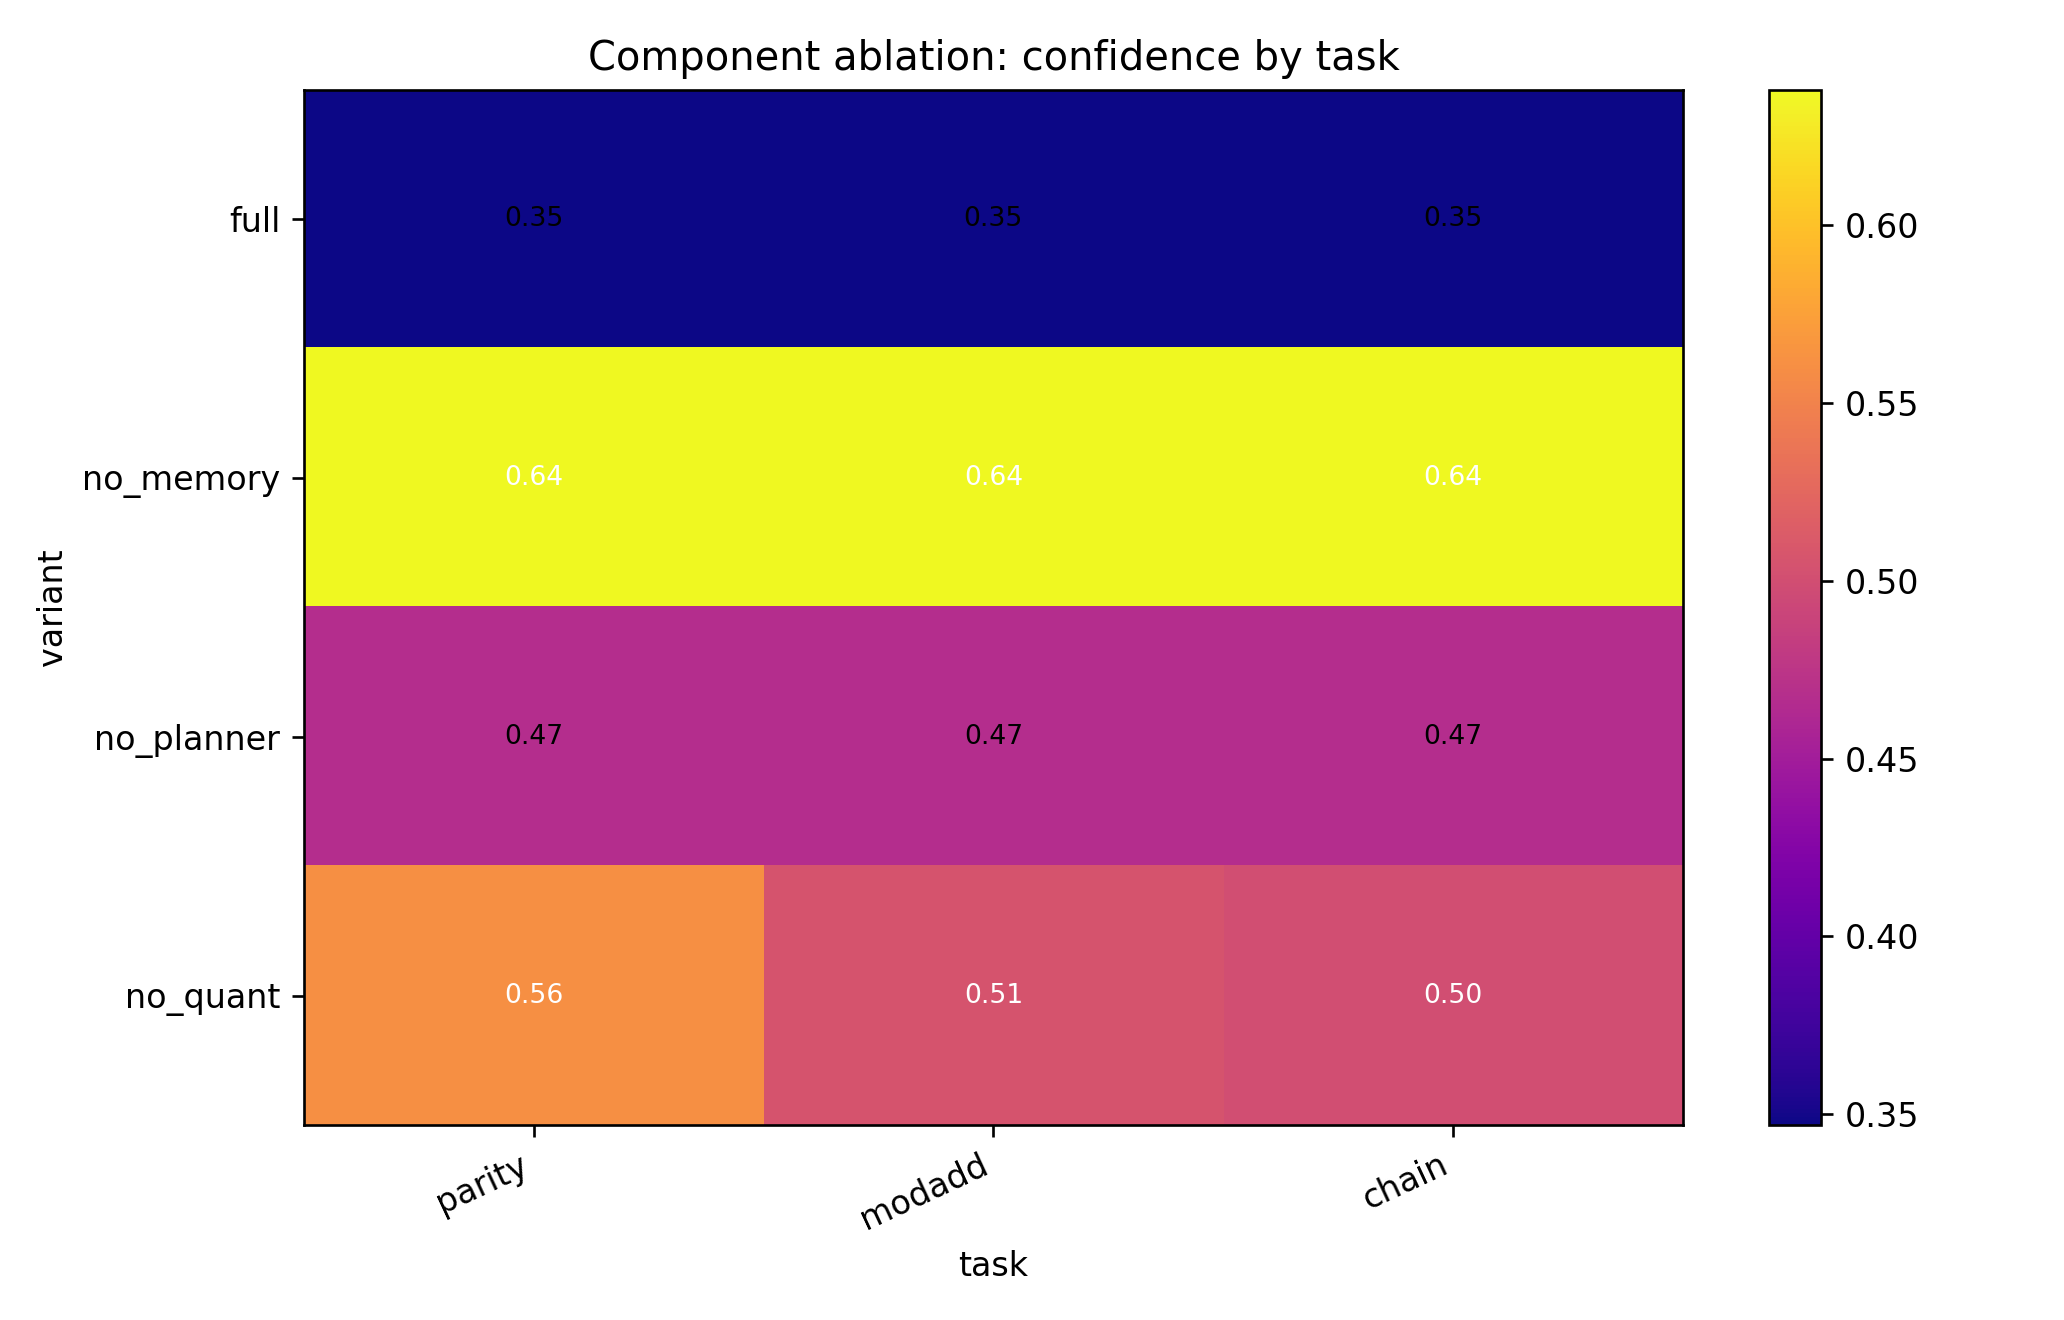
\includegraphics[width=\linewidth]{results/heatmap_variant_confidence.png}
\caption{Confidence by component ablation.}
\label{fig:variant_confidence}
\end{subfigure}
\caption{Component ablation heatmaps for the trained reference model. The memory pathway in particular changes confidence magnitude, while planner removal affects the balance between confidence and task accuracy.}
\label{fig:variant_heatmaps}
\end{figure}

\begin{figure}[t]
\centering
\begin{subfigure}[t]{0.49\linewidth}
\centering
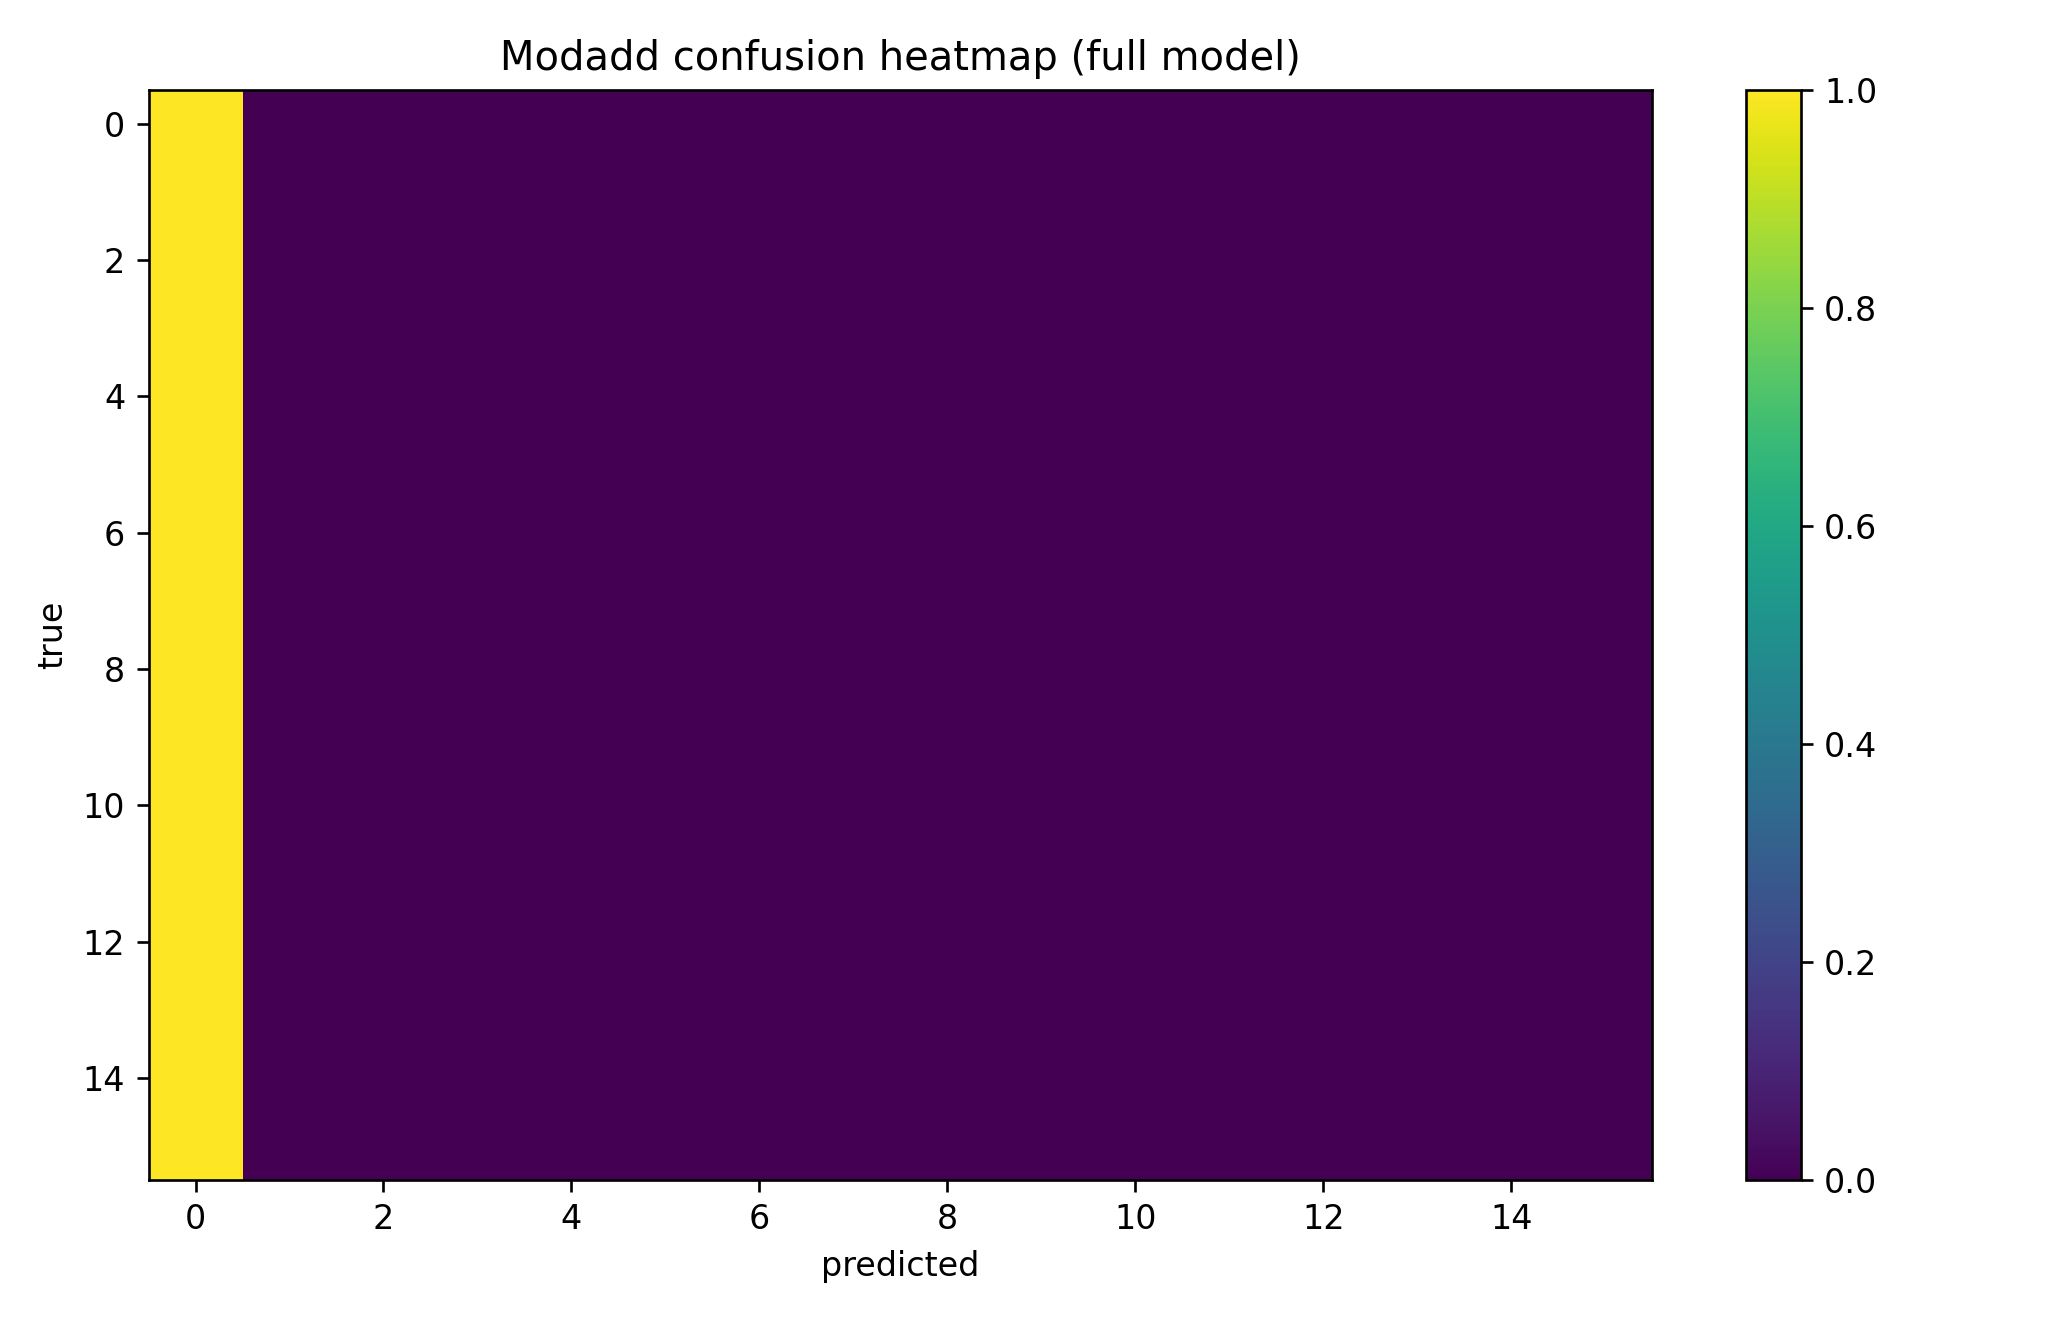
\includegraphics[width=\linewidth]{results/heatmap_modadd_confusion.png}
\caption{Modadd confusion structure.}
\label{fig:modadd_confusion}
\end{subfigure}
\begin{subfigure}[t]{0.49\linewidth}
\centering
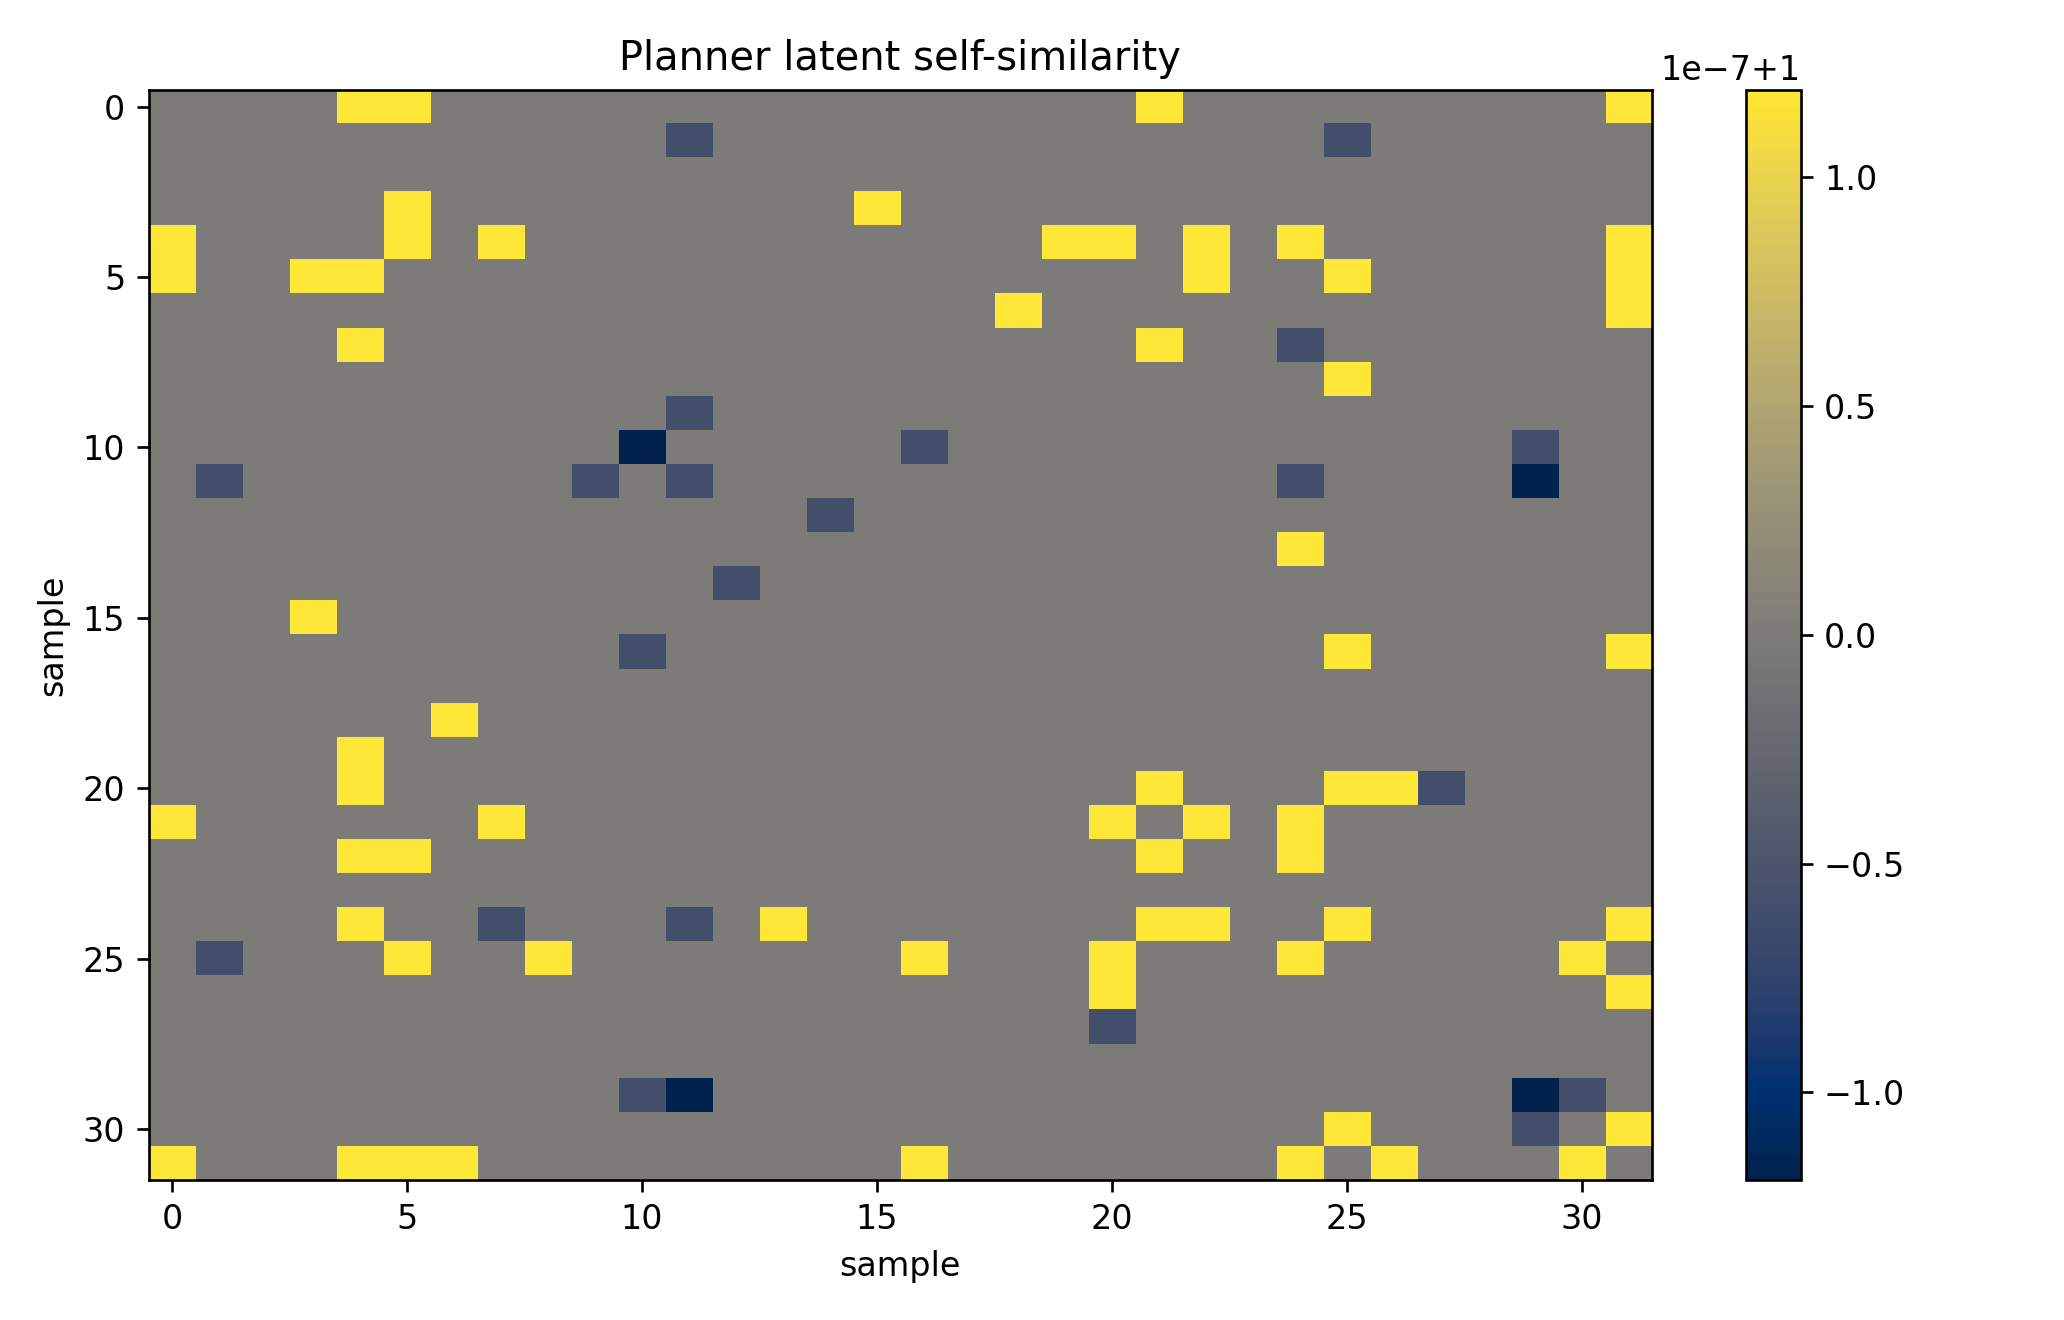
\includegraphics[width=\linewidth]{results/heatmap_planner_similarity.png}
\caption{Latent trajectory self-similarity.}
\label{fig:planner_similarity}
\end{subfigure}
\caption{Structural diagnostics for the full model. The modular arithmetic confusion matrix remains diffuse, which is expected in a smoke-test setting, while the planner similarity matrix retains nontrivial self-similarity structure across latent states.}
\label{fig:confusion_and_plan}
\end{figure}

\begin{figure}[t]
\centering
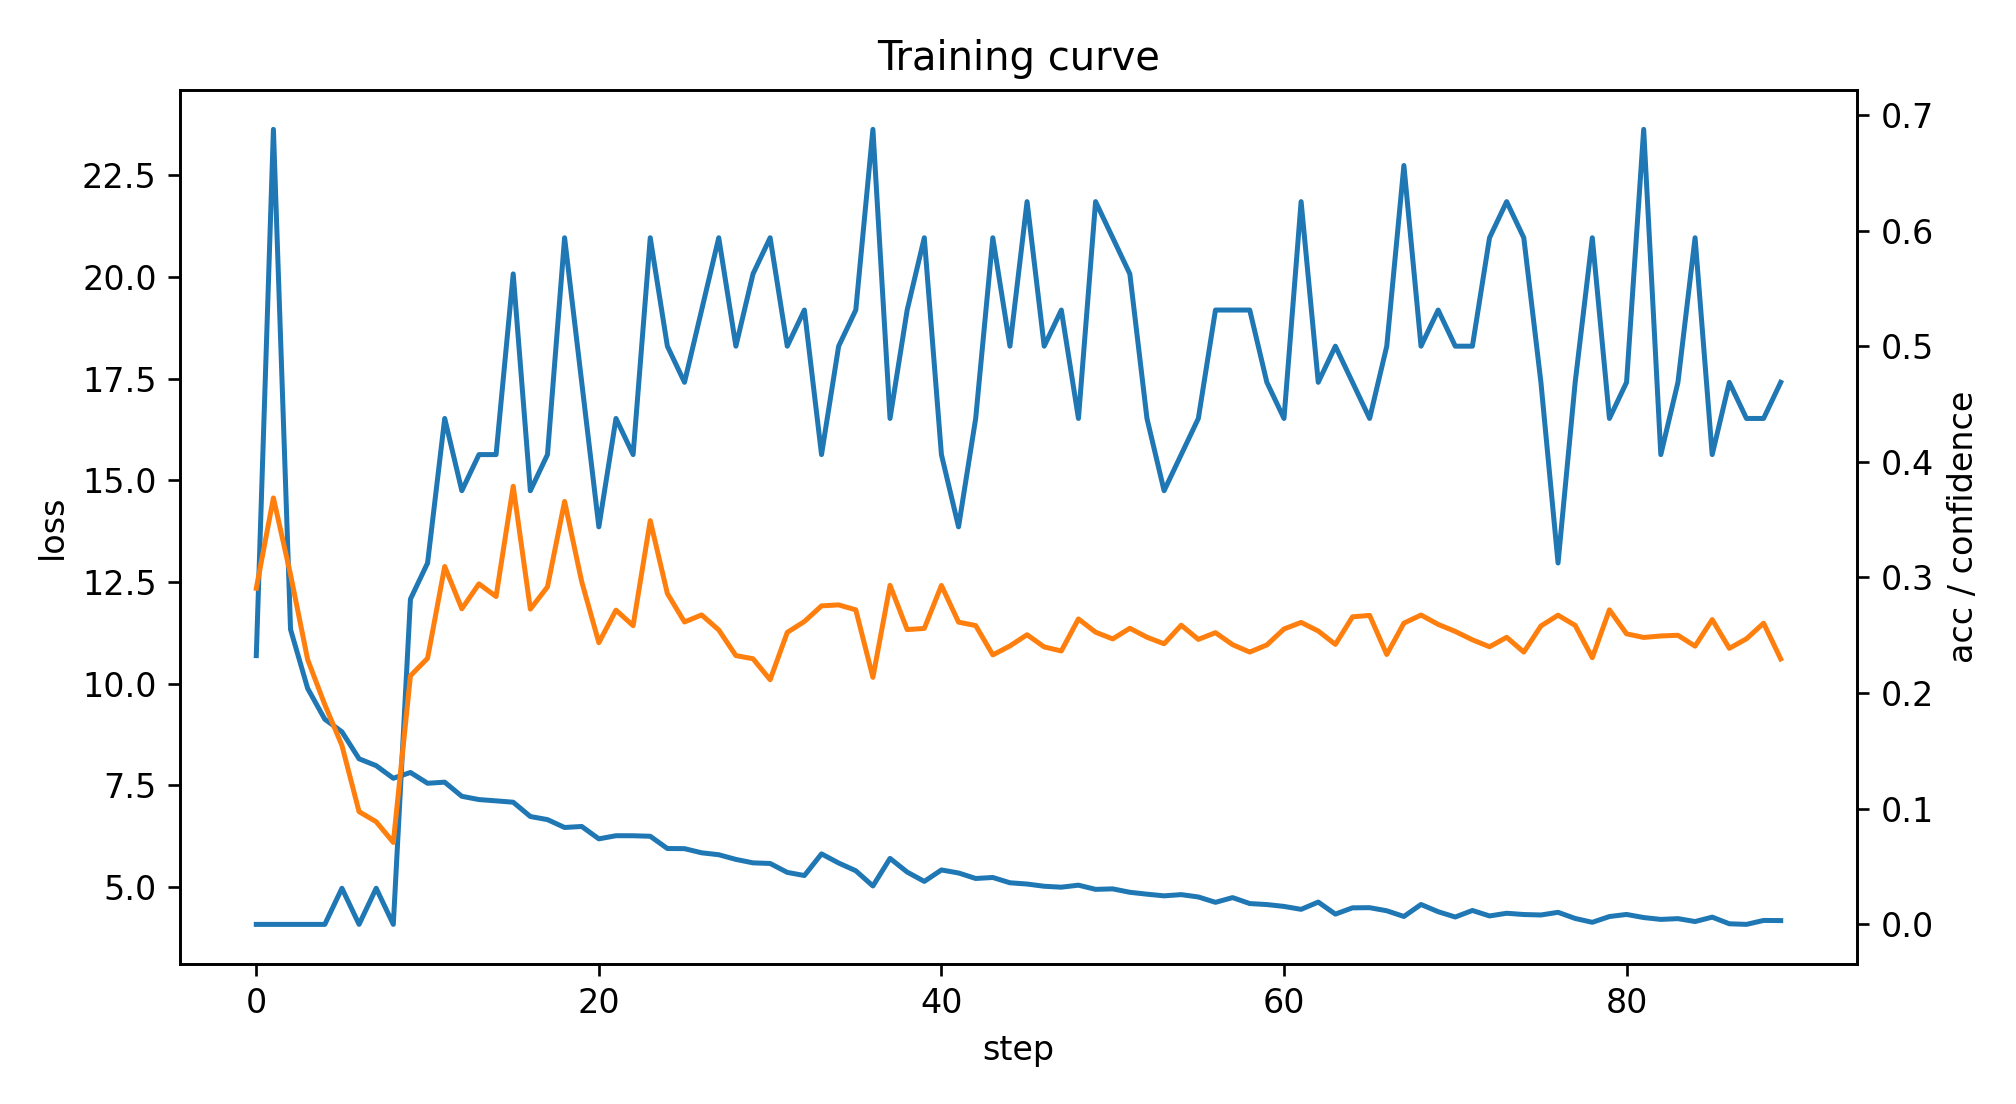
\includegraphics[width=0.88\linewidth]{results/training_curve.png}
\caption{Training curve for the mixed-curriculum smoke test. The curve is intentionally short but still shows a consistent reduction in loss and a noncollapsed confidence trajectory.}
\label{fig:training_curve}
\end{figure}

Taken together, these results support three practical conclusions. First, the repository is operational end to end, since model instantiation, synthetic data generation, short mixed-curriculum training, and visualization all complete successfully. Second, the model remains far from a task-specialized solver, which is expected because the current runs are intentionally short and serve as smoke tests rather than final benchmarks. Third, the latent trajectory and ablation heatmaps are not trivial: they show that memory, quantization, and planning each perturb the system in different ways, and that these perturbations are visible in both confidence behavior and latent similarity structure.

\section{Discussion}

LAM-JEPA is best understood not as a conventional encoder--decoder model, but as a structured latent reasoning system whose internal state is explicitly organized around prediction, correction, and reuse. The key design choice is to represent the solution process as a trajectory in latent space rather than a one-shot mapping from prompt to answer. This makes intermediate solution states available to the model, allows it to distinguish routine cases from atypical ones, and makes the model inspectable through geometric, spectral, and topological tools.

The architecture is intentionally biased toward invariance under surface perturbation while remaining sensitive to structural changes. The latent space is not meant to be merely compact; it is meant to be organized. The geometric regularizer promotes local isometry so that semantically similar reasoning states stay nearby, while the topological regularizer prevents the representation from collapsing distinct reasoning families into a single mode. The spectral branch further strengthens this bias by giving the model access to a complex-valued frequency representation. In mathematical or signal-like tasks, local syntax is often insufficient to resolve the intended reasoning path. Global periodicity, oscillation, cancellation, and phase alignment can be crucial.

The memory module is more than an auxiliary cache. It acts as a selective archive of salient reasoning episodes, and the salience criterion is designed to reflect not just surprise but pedagogical relevance, uncertainty, gradient energy, and topological novelty. The planning module is the bridge between latent dynamics and output generation. It allows the model to search over reasoning trajectories rather than merely emit answers. The value head, uncertainty head, and verifier head jointly provide a decision rule that balances correctness, confidence, and compute cost.

\section{Limitations}
LAM-JEPA assumes access to structured tasks for pretraining and evaluation. It is strongest on domains with exact or semi-exact checking, such as arithmetic and algebra. In open-ended language tasks, the verifier and rubric heads must be complemented by stronger external tools or human judgment. The planning module can be computationally expensive if search depth is large. For deployment, hybrid strategies are recommended: a fast path for routine cases and deeper planning only when uncertainty is high.

\section{Conclusion}
We proposed LAM-JEPA, a latent-action extension of JEPA for adaptive exam reasoning, verification, and grokking-oriented generalization. The system integrates latent representation learning, discrete symbolic compression, world-model planning, sparse engram memory, geometric and topological regularization, confidence estimation, rubric grading, and verification into a single architecture.


\section{References}
\begin{enumerate}[leftmargin=2em,label={[{\arabic*}]}]
\item Assran, H., Duval, Q., Misra, I., Bojanowski, P., Vincent, P., Rabbat, M., \& LeCun, Y. (2023). Self-Supervised Learning from Images with a Joint-Embedding Predictive Architecture. \emph{arXiv preprint arXiv:2301.08243}.
\item van den Oord, A., Vinyals, O., \& Kavukcuoglu, K. (2017). Neural Discrete Representation Learning. \emph{Advances in Neural Information Processing Systems}.
\item Ha, D., \& Schmidhuber, J. (2018). Recurrent World Models Facilitate Policy Evolution. \emph{Advances in Neural Information Processing Systems}.
\item Power, A., Burda, Y., Edwards, H., Babuschkin, I., \& Leike, J. (2022). Grokking: Generalization Beyond Overfitting on Small Algorithmic Datasets. \emph{arXiv preprint arXiv:2201.02177}.
\item Carlsson, G. (2009). Topology and data. \emph{Bulletin of the American Mathematical Society}, 46(2), 255--308.
\item Edelsbrunner, H., Letscher, D., \& Zomorodian, A. (2000). Topological persistence and simplification. \emph{Proceedings of the 41st Annual Symposium on Foundations of Computer Science}.
\end{enumerate}


\end{document}
